\documentclass{article}
%
\usepackage[mathcal,mathbf]{euler}
%\usepackage{theorem,amsmath,enumerate,fancyhdr,amssymb,accents,amsfonts}
\usepackage{theorem,amsmath,enumerate,fancyhdr,amssymb,amsfonts}
\usepackage[pdftex]{graphics}
\usepackage{graphicx}
%% In order to be consistent use the notation in the following style
%% file as much as you can. You may take a look at the file to see
%% what is available.
\usepackage{myDefs}
\usepackage{ulem}
\usepackage{diagbox}


%%
%% Here is where the title goes. Write down lecture number for ?
\title{ 
    Algorithmic Learning Theory\\
    Spring 2017\\
    Lecture 2 %1 or 2 or 3 etc
}
\author{
    {\bf Instructor: } Farid Alizadeh\\
    {\bf Scribe: } Chien-Ming Huang\\
    {\bf Edit: } Yuan Qu\\
}
\date{1/25/2017} %put the date of the lecture here NOT the date the note was written

\begin{document}

\pagestyle{fancy}
\lhead{
    {\bf Scribe:}{Chien-Ming Huang }
    {\bf Edit:}{Yuan Qu}\\
    {\bf Lecture 2}
} %insert lecture number
\rhead{
    {\bf Date: }01/25/2017
} %enter lecture date NOT today's date

\maketitle
%
%%\oddsidemargin 0.0in 
%%\textwidth 6.25in 
%%\topmargin -0.25in 
%%\textheight 8.25in    

%%%%%%%%%%%%%%%%%%%%%%%%%%%%%%%%%%%%%%%%%%%%%%%%%%%%%%%%%%%%%%
%% Below  is where the body of your notes goes.
%%%%%%%%%%%%%%%%%%%%%%%%%%%%%%%%%%%%%%%%%%%%%%%%%%%%%%%%%%%%%%

\medskip
\begin{enumerate}
    \item Review Bayes Theory(Lecture 1) 
    \item Random Variable and Distribution
        \begin{enumerate}
            \item Random variable
                \begin{enumerate}
                    \item DRV, discrete random variable
                    \item CRV, continuous random variable
                \end{enumerate}
            \item Distribution function
                \begin{enumerate}
                    \item CDF, cumulative distribution function
                    \item pdf or pmf, probability density(Mass) function
                \end{enumerate}
            \item Discrete distribution
                \begin{enumerate}
                    \item Discrete uniform distribution
                    \item Beunoulli's distribution
                    \item Binomial distribution
                \end{enumerate}
            \item Continuous distribution
                \begin{enumerate}
                    \item Continuous uniform distribution
                    \item Normal distribution
                \end{enumerate}
        \end{enumerate}
    \item Multivariate Distributions
        \begin{enumerate}
            \item Random vector
            \item Discrete multivariate distribution
            \item Binormal distribution
            \item Marginal distribution
            \item Conditional distribution
        \end{enumerate}
    \item Bayes Classification
\end{enumerate}

%% Write a quick short paragraph summarizing the topic covered in
%% the lecture here. You may use itemization or enumeration
\section{Review Bayes Theory(Lecture 1)}
See notes in "Lecture 1".
\section{Random Variable and Distribution}{
    \subsection{Random Variable}{
        \subsubsection{Discrete Random Variable(D.R.V)}{
            $ x\rightarrow t_1, t_2, \cdots, t_n$
        }
        \subsubsection{Continuous Random Variable(C.R.V)}{
            $ x\rightarrow [a, b]$ a range of value.
        }
    }
    \subsection{Distribution Function}{
        \subsubsection{CDF: }{
            Cumulative Distribution Function\\
            $ F_x(t)= P[x\le t]$, probability can only increase\\

            \begin{enumerate}{
                \item For Discrete:
                    \begin{center}{
                        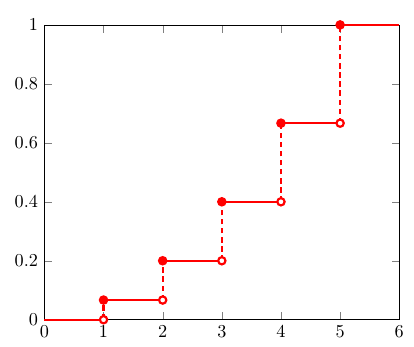
\includegraphics[scale=0.3]{dis-cdf.png}
                    }
                    \end{center} 
                \item For Continuous:
                    \begin{center}{
                        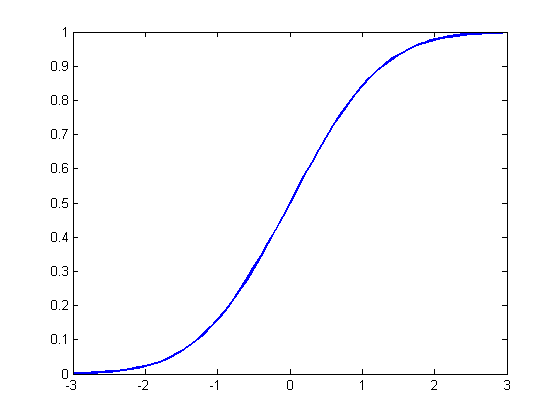
\includegraphics[scale=0.3]{con-cdf.png}
                    }
                    \end{center}  
            }
            \end{enumerate}  
        }
        \subsubsection{pdf or pmf: }{
            Probability Density(Mass) Function\\
            
            \begin{enumerate}{
                \item For Discrete:
                    \[ x: F_x(t)= P[x= t] \]
                    \begin{center}{
                        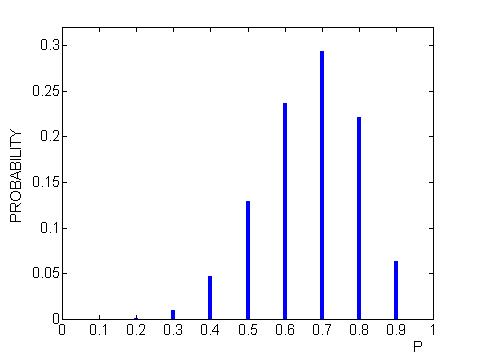
\includegraphics[scale=0.3]{dis-pdf.jpg}
                    }
                    \end{center}
                \item For Continuous: 
                    \[ f_x(t) = \frac{d}{dt}F_x(t), \text{ } F_x(t)=\int_{-\infty}^{t}f_x(t)dt \]
                    \begin{enumerate}[i]{
                        \item $f_x(t)\ge 0$
                        \item $\int_{-\infty}^{\infty}f_x(t)dt= 1$
                    }
                    \end{enumerate}

                    \begin{center}{
                        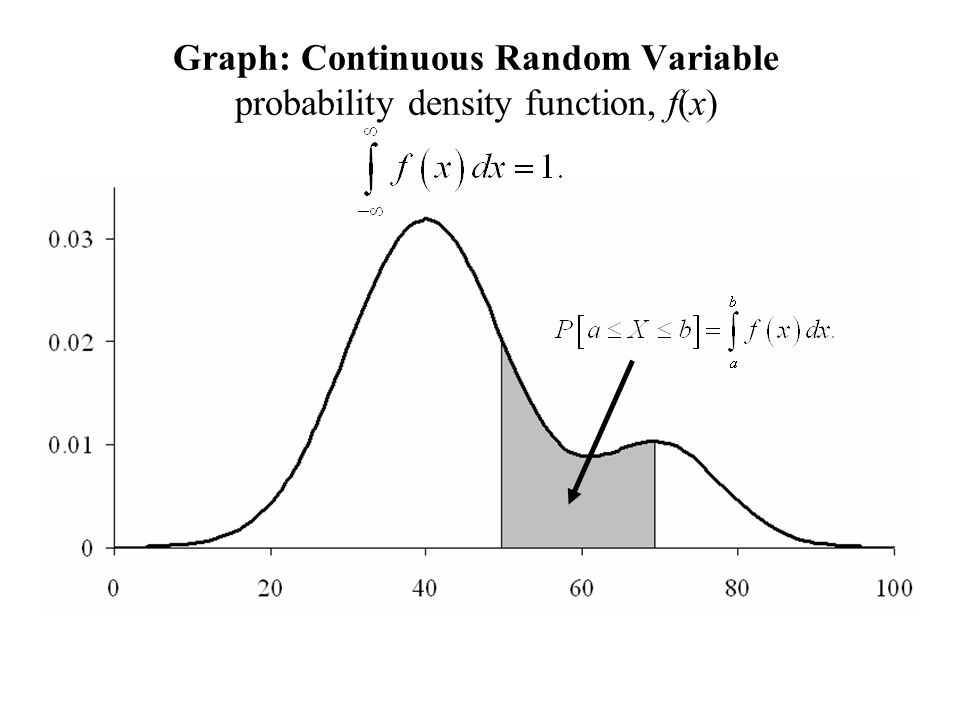
\includegraphics[scale=0.3]{con-pdf.jpg}
                    }
                    \end{center}
            }
            \end{enumerate}  
        }
    }
    \subsection{Discrete Distribution}{
        \subsubsection{Discrete Uniform Distribution}{
            \[ x: 1,2,3, \cdots, k\]
            \[ pdf: u_x(t)= \begin{cases} 
                \frac{1}{n}, & \text{if } t=1, 2,  \cdots, n \\
                0, & \text{otherwise} 
            \end{cases}\]
            \begin{center}{
                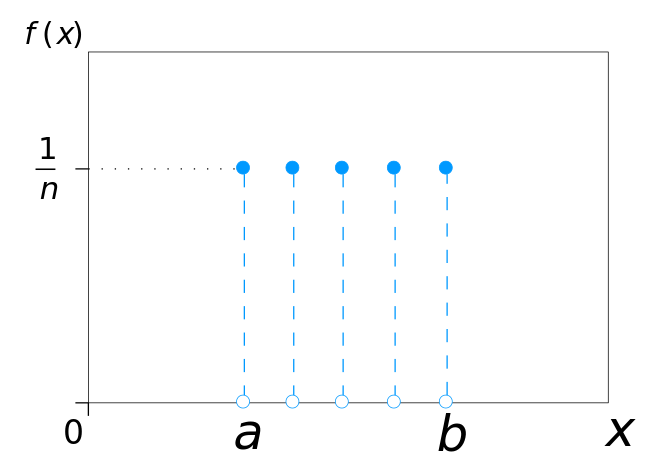
\includegraphics[scale=0.25]{Dis_Uniform_distribution_pdf.png}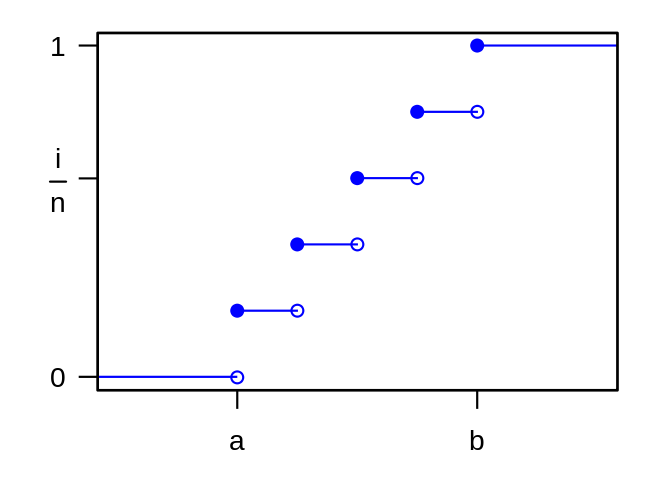
\includegraphics[scale=0.25]{Dis_Uniform_distribution_CDF.png}
            }
            \end{center}
        }
        \subsubsection{Bernoulli Distribution}{
            \[pdf: f_x(t)= \begin{cases} 
                p, & x = 1 \\ 
                1-p, & x = 0 \\
                0, & \text{otherwise}
            \end{cases}\]

            \[CDF: F_x(t)= \begin{cases} 
                0, & x \leqslant 0 \\ 
                1-p, & 0 \leqslant x < 1 \\
                0, & x \geqslant 1
            \end{cases}\]
        }
        \subsubsection{Binomial Distribution}{
            numbers of 0's in independent Bernoulli trial with $P[0]= p$
            \[\text{pdf: } b(t| p, n)= {n \choose t}p^t (1-p)^{n-t}, \text{ } {n \choose t}=\frac{n!}{t!(n-t)!}\]
            \[\text{CDF: } B(t| p, n)= \sum_{n=0}^t b(t| p, n)\]
        }
    }
    \subsection{Continuous distribution}{
        \subsubsection{Continuous uniform distribution}{
            \[ u(t| a, b)= \begin{cases} 
                \frac{1}{b-a}, & a \leqslant t \leqslant b \\ 
                0, & \text{otherwise}
            \end{cases}\]
            \begin{center}{
                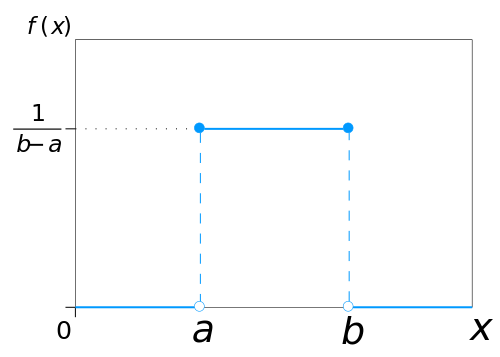
\includegraphics[scale=0.25]{Con_Uniform_distribution_pdf.png}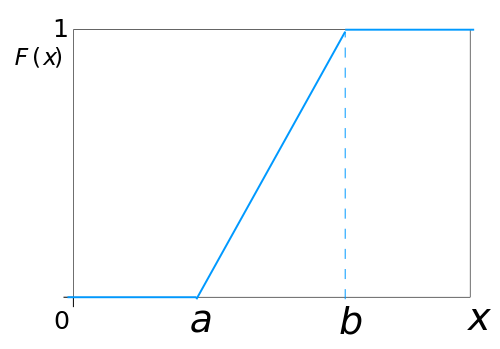
\includegraphics[scale=0.25]{Con_Uniform_distribution_CDF.png}
            }
            \end{center}
        }
        \subsubsection{Normal distribution}{
            mean= $\mu $ and std.= $\sigma $
            \[\text{pdf: } \mathit{f}(\mathit{x}| \mu, \sigma^2)= \frac{1}{\sqrt{2\pi} \sigma }\mathit{e}^{-\frac{(\mathit{x}-\mu)^2}{2\sigma^2}}\]
            \[\text{CDF: } \frac{1}{2} \lbrack 1+erf(\frac{\mathit{x}-\mu}{\sigma\sqrt{2}})\rbrack\]
            \[erf(\mathit{x})=\frac{1}{\sqrt{\pi}}\int_{-\mathit{x}}^{\mathit{x}}\mathit{e}^{-t^2}dt\]
            \begin{center}{
                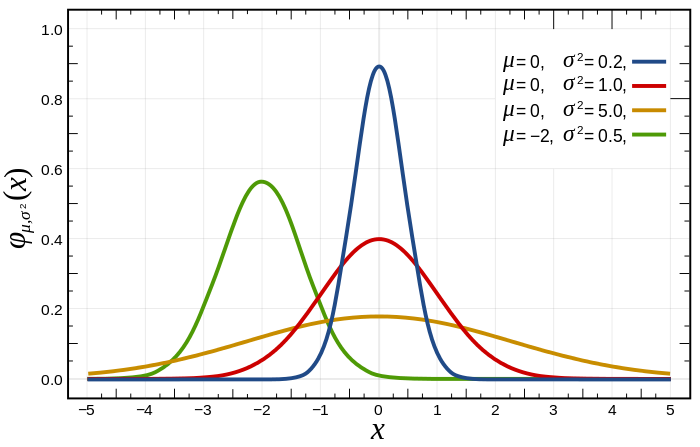
\includegraphics[scale=0.25]{Normal_distribution_pdf.png}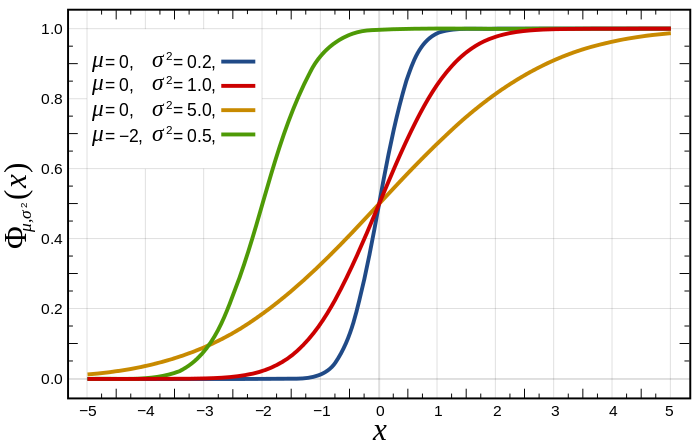
\includegraphics[scale=0.25]{Normal_distribution_CDF.png}
            }
            \end{center}
        }
    }
}
% section Random Variable and Distribution (end)

\section{Multivariate Distributions}{
    \subsection{Random Vector}{
        \(X_N=(x_1, x_2, \cdots x_N)\) can be continuous or discrete.
        \[\text{CDF: } F_x(t_1, t_2, \cdots t_n)= P[x_1\leqslant t_1,x_2\leqslant t_2, \cdots, x_n\leqslant t_n]\]
        \[\text{pdf: } \begin{cases}
            \frac{\partial}{\partial t_1 \partial t_2 \partial t_3 \cdots \partial t_n} F(t_1, t_2, \cdots t_n)= f_{\uwave{x}}(t_1, \cdots, t_n), & \text{all continuous}\\
            P[x_1= t_1,x_2= t_2, \cdots, x_n= t_n]=f_{x}(t_1, \cdots, t_n), & \text{all discrete}
        \end{cases}\]
        both are joint distribution R.V. $x_1, \cdots, x_n$
    }
    \subsection{Discrete Multivariate Distribution}{
        \[ Y\rightarrow 1, 2, \cdots, r; \quad P[Y=r_1]=P_u; \quad \sum P_u= 1\]
        repeat $n$ times, $x_k$= number of times $Y = k$ occurs 
        \[\uwave{x}= (x_1, \cdots, x_n)\]
        \[\text{pdf: } \mathit{f_x}(x_1, x_2, \cdots, x_n) = P[x_1=t_1, x_2=t_2, \cdots, x_n=t_n]{n \choose t_1, t_2, \cdots, t_n}{p_1}^{t_1}{p_2}^{t_2}\cdots{p_n}^{t_n}\]
        \[{n \choose t_1, t_2, \cdots, t_r}= \frac{n !}{t_1! t_2! \cdots t_n!}\]
    }
    \subsection{Binormal distribution}{
        \[\uwave{x}=(x_1,x_2), \text{both continuous}\]
        \[\uwave{\mu}= { \mu_1 \choose \mu_2}, \sigma_1^2 \rightarrow x_1, \sigma_2^2 \rightarrow x_2, \sigma_{21} \rightarrow x_1,x_2 \]
        \[\text{Covariance Matrix: } 
        \Sigma= \begin{pmatrix} 
            \sigma_1^2 & \sigma_{12} \\ 
            \sigma_{12} & \sigma_2^2 
        \end{pmatrix} \]
        \[ \phi(t_1,t_2| \uwave{\mu}, \Sigma)= \frac{1}{\sqrt{2 \pi \cdot Det(\Sigma)}}exp[( \uwave{ t } -\uwave{\mu})^T \Sigma^{-1} (\uwave{t} -\uwave{\mu}),  \uwave{t} ={ t_1 \choose t_2} \]
        \[\phi(t_1)= \int_{-\infty}^{\infty} \phi(t_1,t_2| \cdots) dt_2\]

        Joint pdf: \(f_{(x1,x2)}(t_1,t_2)\)

        In a similar way, for multi-normal distribution, 
        \[ \Sigma= \begin{bmatrix}
            \sigma_1^2 & \sigma_{12} & \sigma_{13} & \cdots & \sigma_{1n}  \\
            \sigma_{12} & \sigma_2^2 & \cdots & \cdots & \sigma_{2n}  \\
            \vdots & \vdots &  \vdots & \ddots & \vdots \\
            \sigma_{n1} & \cdots & \cdots & \cdots & \sigma_{n}^n 
        \end{bmatrix}\]
    }
    
    \subsection{Marginal Distribution}{
        \[ \uwave{x}= (x_1, x_2, \cdots, x_n) \rightarrow f_{x_{\sim}}(t_1, \cdots, t_n)\]
        To calculate pdf,
        \[f_{x_{\sim}}(t_1, t_2, \cdots, t_n) = \int_{t_{k+1}, \cdots, t_n}^{\infty} f_{x_{\sim}}(t_1, \cdots, t_n)dt_{k+1}, \cdots, dt_n= \sum_{t_{k+1}}\sum_{t_{k+2}}\cdots \sum_{t_{n}}f_{x_{\sim}}(t_1,\cdots, t_n)\]
        
        Joint pdf: \(f(t_1, t_2)\)
    }

    \subsection{Conditional Distribution (2 Vars)}{
        \[\uwave{x}=(x_1, x_2) \rightarrow \text{ joint:} f(t_1,t_2)\]
        Conditional distribution means: \(\mathit{f}_{x_1|x_2}(t_1|t_2=\mathit{a})\), \(\mathit{a}\) is a given constant, \(\mathit{x}_2\) is given, fixed.

        \[f_{x_1|x_2}(t_1|t_2)=\frac{f_{x_{\sim}}(t_1,t_2)}{f_{x_2}(t_2)}\]
        By defination, \(f_{x_{\sim}}(t_1,t_2)\) is joint distribution, \(f_{x_2}(t_2)\) is marginal distribution. And, we have,

        \[f_{x_{\sim}}(t_1, t_2)=  f_{x_1|x_2}(t_1|t_2)f_{x_2}(t_2)\]
        \[f_{x_2|x_1}(t_2|t_1)=\frac{f_{x_{\sim}}(t_1,t_2)}{f_{x_1}(t_1)}\]
        \[f_{x_{\sim}}(t_1, t_2)=  f_{x_2|x_1}(t_2|t_1)f_{x_1}(t_1)\]

        So, 
        \[f_{x_1|x_2}(t_1|t_2)=\frac{f_{x_2|x_1}(t_2|t_1)f_{x_1}(t_1)}{f_{x_2}(t_2)} \rightarrow \text{Bayes Rule}\]

        \paragraph{e.g. }{
            \begin{tabular}{l|*{4}r}
                \hline
                \diagbox{$x_2$}{$x_1$} & 1& 2 & 3 & $f_{x_2}(t)$\\
                \hline
                0 & 0.1 & 0.4 & 0.2 & 0.7 \\
                \hline
                1 & 0.2 & 0.05 & 0.05 & 0.3 \\
                \hline
                $f_{x_1}(t)$ &0.3 & 0.45 & 0.45 & \\
            \end{tabular}

            \[P[x_2= 0] = P[x_2=0 \vert x_1=1]+P[x_2=0 \vert x_1=2]+P[x_2=0 \vert x_1=3]=0.7\]
            \[P[x_2= 1] = 1 - P[x_2= 0] = 0.3\]
        }
    }
}
% section Multivariate Distributions (end)

\section{Bayes Classification}{
    \[f_{x_1|x_2}(t_1|t_2)=\frac{f_{x_2|x_1}(t_2|t_1)f_{x_1}(t_1)}{f_{x_2}(t_2)} \rightarrow \text{Bayes Rule}\]

    For discrete: \(f_{x_2}(t_2)= \sum_{t_1}f_{x_2|x_1}(t_2|t_1)f_{x_1}(t_1)\)\\

    For continuous: \(f_{x_2}(t_2)= \int_{-\infty}^{\infty}f_{x_2|x_1}(t_2|t_1)f_{y_1}(t_1)dt\)

    \paragraph{e.g. Height}{
        Supposed that: $x_1 \rightarrow$ Height, $x_2 \rightarrow$ Gender,
        \(\begin{cases} 0  & \text{male} \\ 
        1& \text{female} \end{cases}\)

        For \(x_2= 0 \rightarrow \text{Height} \sim N(69,4.5) \Leftrightarrow f_{x_1|x_2}(t_1|t_2= 0)\phi( t_1|\phi=69, \sigma= 4.5)\)\\

        For \(x_2= 1 \rightarrow \text{Height} \sim N(65,4.2)\Leftrightarrow f_{x_1|x_2}(t_1|t_2= 1)\phi( t_1|\phi=65, \sigma= 4.2)\)\\
            
        Marginal distribution of height for people:
        \[f_{x_1}(t_1)=f_{x_1|x_2}(t_1|t_2= 0)*f_{x_2}(0)+f_{x_1|x_2}(t_1|t_2= 1)*f_{x_2}(1)\]
        \[= \phi(t_1|69, 4.5)\cdot 0.5+\phi(t_2|65, 4.2)*0.5\]
        \[= \phi(t|\frac{69+65}{2},\sqrt{\frac{4.5^2+4.2^2}{2}} )\]

        A person has height 6'7", caculate the probability of each gender.
        \[f(x_2= 0| x_1=67)=\frac{ f_{x_1|x_2}(67|x_2= 0)f_{x_2}(0)}{f_{x_1}(67)}=\frac{\phi(67|69,4.5)\cdot 0.5}{f_{x_1}(67)}\]
        \[f(x_2= 1| x_1=67)=\frac{ f_{x_1|x_2}(67|x_2= 1)f_{x_2}(1)}{f_{x_1}(67)}=\frac{\phi(67|65,4.2)\cdot 0.5}{f_{x_1}(67)}\]
    } 

    \[\text{Loss}(\hat{f}, \uwave{x}|f), \rightarrow \text{Minimum} E_x: Loss (\hat{f}|f)\]
    Misclassification Rate: loss\((\hat{f}, \uwave{x}|f): \begin{cases} 
        0, &\  f_x=\hat{f}(x) \\ 
        1, &\  f_x \ne \hat{f}(x) 
    \end{cases}\), Risk = \(E_x[loss(\hat{f}, \uwave{x}|f)]\)\\

    Probability of Misclassification: \(E_x= \begin{cases}
        \sum_{t_i}t_if_x(t_i), &\   \text{for discrete} \\
        \int_{0}^{1}t\int_{x}(t)dt, &\  \text{for continuous}
    \end{cases}\)

    Bayes Classification Rule for Binary: choose $k$ that $P[y=k|\uwave{x}]$,
    \[k= \underset{k}{\mathrm{argmax}}\frac{P[x|k]P[k]}{P[x]} \propto P[x|k]P[k]\]

    For cost matrix C, assumed that
    \[C_{ij}= \text{the cost of classification } i \text{by wrong classified in } j\]
    \[E_x(loss(j=\hat{f}(x)|i)= \sum_{i=1}^{k}P[i|x]C_{ij} = \sum_{i=1}^{k}\frac{f(x|i)P[i]C_{ij}}{f_x} \cdot C_{ij}\]
    \[ \propto \sum_{i=1}^{k}f(x|i)P[i]C_{ij}\]
}

us 
\\
\\Example: In a box $\frac{1}{4}$ of coins are fake, $\frac{3}{4} $ of coins are real
\\The probability to get fake: $P_r[head]= \frac{1}{3}, P_r[tail]= \frac{2}{3} $
\\The probability to get real: $P_r[head]= \frac{1}{2}, P_r[tail]= \frac{2}{2} $
\\Take a random coin selected, n= 20 times, t= 7 heads, what is $P_r[real]$? what is $P_r[false]$?
\\$x_1$= number of heads in n= 20 trials
\\$x_2= \begin{cases} 0, \text{fake}  &\  f_{x_2}(0)=\frac{1}{4} \\ 
	1, \text{real}  &\  f_{x_2}(1)=\frac{3}{4} \end{cases}$
\\$f(t_2= 0| x_1=7, n= 20)=\frac{f_{x_1|x_2}(7|fake, n= 20)*f_{x_2}(0)}{f_{x_1}(7)}= {20\choose 7}\frac{1}{3}^7\frac{2}{3}^13*0.25=0.45$
\\$f(t_2= 1|x_1=7, n= 20)=\frac{ f_{x_1|x_2}(7|real, n= 20)*f_{x_2}(1)}{f_{x_1}(7)}{20\choose 7}\frac{1}{2}^7\frac{1}{2}^13*0.75=0.55$	

\subsection{Bayes Classfication} 	

\subsection{Modify Bayes Rule(Uneven Cost)} 
$c= avgmin\sum_{i=1}^{k}f(x|i)P_r[i]C_{ij}$
\\Example: Real and Fake: $C=\begin{pmatrix} 0 & 1 \\ 4 & 0 \end{pmatrix}$
\\real:$P_r[x_2=1|x_1=7]*C_{11}+P_r[x_2=0|x_1=7]*C_{12}$
\\fake:$P_r[x_2=1|x_1=7]*C_{21}+P_r[x_2=0|x_1=7]*C_{22}$
\\$min:\begin{cases} 0.55*0+0.45*1=0.45 \\ 
	0.55*4+0.45*0=1.8 \end{cases}$

\end{document}  